\section{Introduction}
Iterative algorithms and recursive programs widely exist in data analytics fields. It is also necessary to parallelize or distribute the iterative computation for processing large scale data. However, the parallelization of algorithms requires programmers to have a rich knowledge of distributed systems. A large number of big data analysis systems have been proposed which provide high-level language for expressing the iterative computation logic \cite{Dean:2004:MSD:1251254.1251264,giraph,maiter,Fan:2017:PSG:3035918.3035942,Malewicz2010Pregel,DBLP:journals/corr/GonzalezBJFHGS15,8017445,Low:2012:DGF:2212351.2212354,Han:2015:GUB:2777598.2777604,grace}.

%Even so, these systems still require the users to understand the specific programming logic. For example, Pregel \cite{Malewicz2010Pregel} adopts the Bulk Synchronous Parallel (BSP) computing model and a vertex-centric programming model, which requires programmers to write vertex-centric programs and explicitly manage the communication.

\begin{comment}
{\color{red}
New interest has recently re-emerged around Datalog for a wide spectrum of knowledge-oriented applications \cite{Aref:2015:DIL:2723372.2742796,7840589,Shkapsky:2013:GQN:2536274.2536290,Alvaro:2010:DDT:2185923.2185942,Shkapsky:2016:BDA:2882903.2915229,Lam:2013:SDE:2510649.2511289,Seo:2013:DSD:2556549.2556572,Wang:2015:AFR:2824032.2824052}%Bigdatalog 25,27,64,47,49}.\begin{comment}
{\color{red}Datalog is an excellent candidate language for large-scale data analytics because of its high-level declarative semantics and support for recursion. Datalog's support for recursion makes the expression of data analysis natural \cite{}{\color{red}which paper}  and its high-level semantics makes it amenable to parallelization and optimization \cite{}{\color{red}which paper}.

In recent years, many system research efforts have raised to improve performance  and scalability based on Datalog systems. Socialite \cite{Lam:2013:SDE:2510649.2511289,Seo:2013:DSD:2556549.2556572} provides a large scale graph evaluation system supporting both sequential and distribute environment. In Socialite, users can define recursive aggregate functions which, as long as they are meet operations, can be evaluated incrementally and efficiently. The \cite{7113340} project provides a full Datalog language implementation and seeks to provide  system supports that optimizes execution over diverse platforms including sequential implementations \cite{Shkapsky:2016:BDA:2882903.2915229}, multi-core machines, and clusters \cite{Shkapsky:2016:BDA:2882903.2915229}. It supports relational algebra, aggregation, and recursion, as well as a host of declarative optimizations. MyriaX \cite{Halperin:2014:DMB:2588555.2594530} implements a Datalog System on share-nothing engines based on Myria \cite{Halperin:2014:DMB:2588555.2594530}. The computations are incremental, and it support s a variety of iterative models (synchronous, asynchronous, different processing priorities) and failure-handling techniques. It is worth mentioning that MyriaX supports asynchronous processing and shows promising performance for some applications, but it fails to tell in which cases asynchronous processing is suited.
}
\end{comment}

Synchronous (sync.) processing and asynchronous (async.) processing are two basic parallel execution strategies for iterative processing. Many sync. processing based parallel/distributed systems \cite{Malewicz2010Pregel,Dean:2004:MSD:1251254.1251264,giraph,maiter,Fan:2017:PSG:3035918.3035942,Malewicz2010Pregel,8017445,Low:2012:DGF:2212351.2212354} as well as async. systems \cite{Low:2012:DGF:2212351.2212354, Tian:2013:TLV:2732232.2732238, Han:2015:GUB:2777598.2777604, grace, ppopp2017} have emerged in recent years. Sync. mode requires expensive synchronization cost and forces computation to execute sequentially, which works against the goal of parallelism. Compared with sync. iteration, async. iteration has many advantages, such as fast convergence \cite{maiter}, more efficient resource utilization \cite{priori-cidr}, and the ability of using priority scheduling. \cite{Zhang:2011:PDF:2038916.2038929}. However in practice, sync. systems are more popular than async. systems. This is because that async. computation suffers from the following three drawbacks:

First, \textbf{Non-guaranteed Correctness}. There are several prior works that have employed async. engine for improving performance \cite{Low:2012:DGF:2212351.2212354, Tian:2013:TLV:2732232.2732238, Han:2015:GUB:2777598.2777604, grace, ppopp2017}. However, these systems only implement asynchronous execution of parallel/distributed algorithms, without any correctness guarantee of the results \cite{Low:2012:DGF:2212351.2212354}. Async. modes are blindly used and may result in inconsistent results for \emph{convex functions}. Maiter \cite{maiter} provides the sufficient conditions for correct async. computations, but these conditions are given in the context of vertex-centric graph computations.
%Programmers should judge the conditions manually by themselves.
%Recursive Algorithm usually has ununified computing expression.Even if the correctness condition are given,it is still difficult to check it from variety handwrite program with different style. Not to say convert the normal program into asynchronous formulation.It seems that we need an high-declarative language to express the computing logic.

Second, \textbf{More Complexity}. Programmers are used to write sequential programs or sync. parallel programs. Had the asynchronization conditions been formally given, it is still hard for a non-expert programmer to manually verify these conditions from their programs. In addition, writing async. programs and debugging async. systems are even harder, because async. implies disorganized and as a result complicated. Experience from Google \cite{Malewicz2010Pregel} strongly suggests a sync. programming model, since async. code is a lot harder to write, tune, and debug.

Third, \textbf{Unstable Performance}. As pointed out in \cite{Xie2015SYNC}, the performance of sync. mode and async. mode varies significantly with different iterative computations, data partitioning methods, execution stages, input datasets, and cluster environments, and no single mode consistently outperforms the other. Even though async. iteration has many advantages over sync. iteration, async. iteration may result in \emph{stale} computations (i.e., processes triggered by messages that soon become stale due to more up-to-date messages) \cite{Fan2018Adaptive}. Stale computations are often redundant and increase unnecessary computation and communication costs. These costs may degrade the performance.

%Xie \emph{et al.} \cite{Xie2015SYNC} and Fan \emph{et al.} \cite{Fan2018Adaptive} have proposed to use a sync./async. hybrid way to maximize the advantages of these two modes.

%Third, \textbf{More Complexity}. Programmers are used to write sequential programs or synchronous parallel programs. So writing asynchronous programs and designing asynchronous systems are even harder, because asynchronous implies disorganized and as a result complicated. Experience from Google \cite{}{\color{red}which paper} strongly suggests a synchronous programming model, since asynchronous code is a lot harder to write, tune, and debug.

%{\color{red}
%Third, \textbf{Unstable Performance}. Asynchronous iterative processing avoids the intermediate result coordination phase. The parallel executions of operations are not synchronized and not strictly ordered. This implies that the computations and communications are not under control any more, which may lead to stale computations/communications and potentially reduces the efficiency. The performance gain from asynchronous computation may be not enough to compensate for the performance loss from stale computations/commmunications, leading to unstable performance.
%}

To address the first concern on correctness, we seek to find the root reason of incorrectness. In parallel computing, the inputs of \textbf{aggregate operation} need to be synchronized. All the inputs of aggregation should be ready before aggregation can be started. Given an iterative computation or recursive program with aggregation in each iteration or recursion, the synchronization is required in each iteration to guarantee the correctness of aggregation. However, motivated by our observation, we has studied that a broad class of iterative/recursive algorithms with aggregation do return the correct results when they are executed asynchronously, e.g., Single Source Shortest Path (SSSP) and Connected Components (CC). We analyze the properties of aggregate and non-aggregate operations, and provide the sufficient conditions that guarantee the correctness of async. execution. Even though some iterative computations do not originally satisfy the sufficient conditions, they can be equally converted to new forms such that they are qualified for correct async. execution. For instance, Pagerank, Simrank, Jacobi Method, these iterative algorithms can be equally converted to have new update functions for correct async. execution.


%We observe that a broad class of recursive algorithms with accumulated (or monotonic) recursive aggregation have the possibility of returning the correct results. For example, CC, SSSP, computing paths in DAG,... algorithms are accumulated recursive programs. Given an accumulated recursive program that is composed of interleaving aggregate and non-aggregate operations, as long as the aggregate operation has the commutative property and the aggregate operation and non-aggregate operation have order-independent property, it will return the same result with synchronous processing after enough number of updates. A large class of recursive programs can be rewritten in an accumulated/monotonic form. Even though some cannot, we provide the conditions for converting them. For instance, Pagerank, Belief Propagation, Simrank, Jacobi Method... algorithms that are not originally in the monotonic form can be converted.

To address the second concern on complexity, our idea is exploiting the above correctness conditions to achieve automation. Since the correctness conditions are relied on the properties of aggregate/non-aggregate operations, we need a condition verification strategy that automatically checks the properties of aggregate/non-aggregate operations. The first step is to extract the aggregate/non-aggregate operations from user's recursive program. We choose Datalog \cite{} as user's language because of its high level declarative semantics and its ease of extracting aggregate operation \cite{Shkapsky:2016:BDA:2882903.2915229}. Given the extracted aggregate/non-aggregate operations and the above correctness conditions, the feasibility of async. processing can be automatically verified with the help of a Satisfactory Module Theory (SMT) solver Z3 \cite{DeMoura:2008:ZES:1792734.1792766}. Supposing this program is qualified for correct async. execution, we further propose an automated asynchronization strategy, which can translate a user's Datalog recursive program to an async. parallel/distributed Java program running on multicore machine or on a cluster. To achieve this automation, we build an async. program template. A code generator then uses the extracted aggregate/non-aggregate operators to fill the template and generates async. shared-memory or shared-nothing programs.


%we first propose a condition verification strategy that can automatically verify the feasibility of async. processing. We choose Datalog \cite{} as user's language because of its high level declarative semantics and support for recursion \cite{Shkapsky:2016:BDA:2882903.2915229}. User's Datalog program is first parsed, and the aggregate and non-aggregate operators used in each iteration are extracted. Given the set of sufficient conditions on aggregate/non-aggregate operators, user's recursive Datalog program is automatically checked for verifying whether it can be correctly asynchronized. The automated verification is achieved with the help of a Satisfactory Module Theory (SMT) solver Z3 \cite{DeMoura:2008:ZES:1792734.1792766}.

To address the third concern on performance, the existing work PowerSwitch \cite{Xie2015SYNC} and GRAPE+ \cite{Fan2018Adaptive} have proposed to use a sync./async. hybrid way that adaptively switches a graph-parallel program between sync. mode and async. mode for optimal performance. PowerSwitch \cite{Xie2015SYNC} periodically evaluates the potential benefit from a mode switch and then performs the sync./async. switch based on the evaluation results. GRAPE+ \cite{Fan2018Adaptive} goes further by allowing each worker to decide its own ``mode'' based on its relative progress. Fast workers may follow sync. mode within a group, while meanwhile, the other workers may adopt async. mode. It dynamically adjusts the message sending delay to achieve BSP (sync.), AP (async.), and SSP (between sync. and async.). However, GRAPE+ leverages block-centric programming model so that the adjustment is only executed after each block processing. This may delay the up-to-date messages and limit the benefit of async. processing. We leverage the vertex-centric model and aim to find a more fine-grained adaptive approach to maximize the benefit of async. processing. We observe that the stale computations only degrade performance when computation resources are not enough. This motivates us to feed messages according to computation resources since only new messages could trigger computations. We propose a dynamic buffer scheme that adaptively adjusts the buffer size by monitoring the heaviness of workload on each worker. By this way, the degree between async. and sync. on each worker can be adaptively tuned in a more fine-grained way.

%The stale computations that degrade async. performance can be attributed to the frequent communications. The frequency of async. communication has the potential to determine the degree of asynchrony. More frequent communication leads to more frequent updates, as a result more asynchrony. More asynchrony can accelerate convergence but may result in stale computation costs, which outweighs the gain. In contrast, less frequent communication accumulates more messages and performs ``bigger'' updates. The extreme is that all workers do not communicate with each other until all workers have processed their own assigned data, which is exactly sync. iteration. Based on this observation, we propose a dynamic buffer scheme to buffer the messages. It can adaptively adjust the buffer size by monitoring the heaviness of workload. The idea behind is to feed messages according to computation resources, since the stale computations only degrade performance when computation resources are not enough. By this way, the degree between async. and sync. can be adaptively tuned for optimal performance.


%. They develope GRAPE+ with SSP/BSP/AP hybirded.% While none of these work concerned about improving the performance of asynchronous processing.
%In distributed environment, the network cannot tolerate fully real-time communication. So previous asynchronous processing system choose to using message buffer strategy to avoid frequent communication. In traditional opinion, message buffer size should be setted as small as possible under network restriction to speedup the information update.  However according to our work, too fast updating is not always effective, since it may incur stale or invalid computation. So the optimal buffer size for different workload is not fixed. Even within one running cycle, the optimal buffer size is also dynamic changing. But none of the previous work discussed this. So in this paper, we proposed a dynamic buffer strategy. Different from the previous work, we use only asynchronous mode with dynamic buffer, which realized similar function with previous work and only introduced little overhead.
%Our system is able to automatically check whether a recursive Datalog program can return correct result with asynchronous recursive execution from user's Datalog program. This is achieved by automated sufficient conditions verification using Z3 smt solver.
%A3Log can also automate the conversion for some algorithm that satisfied the convertible condition without user's participation. Further, A3Log provides both shared-memory runtime engine and distributed runtime engine for fast execution.


%We propose the correctness conditions based on the analysis of aggregate and non-aggregate operations.

%n an iterative computation can be abstracted into a series of non-aggregate and aggregate operations.Aggregate operation is known to be hardly parallelized{\color{red} which paper} \cite{distribute aggregate from ms}, while non-aggregate operation can be embarrassingly parallel.

%First,we abstract the iterative computation into recursive aggregation program. And then we  Then we proposed accumulate recursive aggregation and defined the conversion conditions from normal recursive aggregations. Then we generalized the Further some unsatisfiable algorithm, can even be automatically converted to the asynchronous program with our convertible schema.

%we also design and implement a Datalog system supporting automated asynchronous execution, A3Log.We choose Dalalog as its high level language because of its high-level declarative semantics and support for parallel recursion{\color{red}which paper}\cite{}. Our system is able to automatically check whether a recursive Datalog program can return correct result with asynchronous recursive execution from user's Datalog program. This is achieved by automated sufficient conditions verification using Z3 smt solver.
%A3Log can also automate the conversion for some algorithm that satisfied the convertible condition without user's participation. Further, A3Log provides both shared-memory runtime engine and distributed runtime engine for fast execution.


%Maiter \cite{maiter} provides the sufficient conditions for asynchronous graph processing,but these conditions are not generalized enough and only suit for several graph algorithm. In this paper, we generalize the sufficient conditions which can be easily identified from  user's Datalog program. %Aggregate operation is known to be hardly parallelized \cite{distribute aggregate from ms}, while non-aggregate operation can be embarrassingly parallel.% Synchronization of parallel computations seems to be the unavoidable coordination step for correct aggregation result though it is known costly.
\begin{figure}[t]
    \centerline{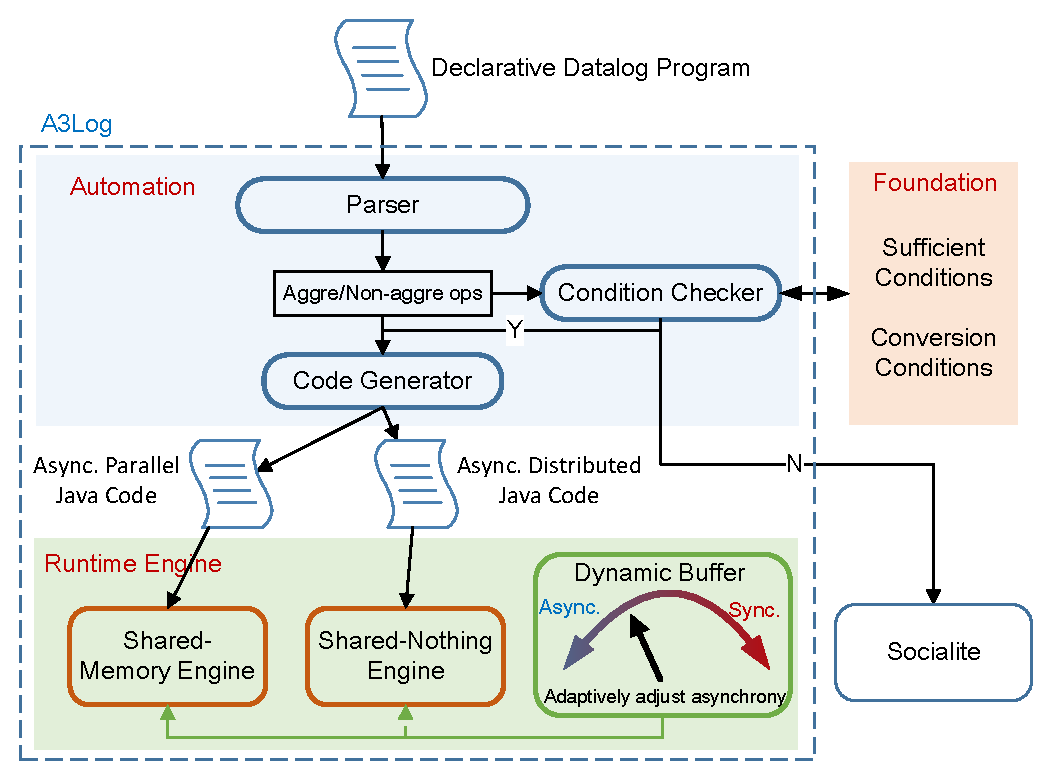
\includegraphics[width=3in]{fig/intro.eps}}
    \caption{A3Log summarization.}
    \label{fig:intro}
\end{figure}


To integrate all the above techniques, we design and implement a parallel/distributed Datalog system \emph{A3Log} that supports Automated Asynchronous Aggregation. As shown in Fig. \ref{fig:intro}, user's submitted Datalog program is first analyzed by \textit{Parser} such that the aggregate/non-aggregate operators are extracted. \textit{Condition Checker} then analyzes the properties of aggregate/non-aggregate operators to verify the feasibility of async. execution by using Z3 SMT solver \cite{}. If the program is qualified for async. execution, \textit{Code Generator} will use the extracted aggregate/non-aggregate operators to generate async. parallel/distributed Java programs according to the async. code template. Otherwise, the program is sent to the Socialite runtime engine for synchronous evaluation. We also implement a shared-memory engine running on multicore machine and a shared-nothing engine running on cluster. The async. Java program is then executed on the parallel/distributed runtime engine. Our dynamic buffer scheme in runtime engine will adaptively adjust the degree of asynchrony to help achieve better performance.


The contributions of this paper are summarized as follows.
\begin{itemize}
	%{\color{red}\item To guarantee the correctness of recursive Datalog program, we proposed a series of conditions of converting  recursive aggregation into a self-defined \textbf{Accumulative Recursive AgGregation}. Moreover new sufficient conditions that guarantee asynchronous processing to return the same result as synchronous processing. which has proposed based on the analysis  of aggregate and non-aggregate operators in ARAG.Even for some recursive programs that do not satisfy these conditions, we propose an approach to conditionally convert them to be qualified for asynchronous aggregation.}
	%\item Correctness. We define the accumulated recursive aggregation (ARA) that has the possibility of returning correct results when executing asynchronously. We also propose the convert conditions from normal recursive aggregation (NRA) to ARA. Furthermore, based on the analysis of aggregate and non-aggregate operations' properties, we provide the conditions for correctly converging to the result when asynchronously executing ARA.	
	%\item Automation. To alleviate the burden of programmers, we propose an automated condition verification technique by leveraging satisfiability modulo theories (SMT). User's accumulated recursive program (ARP) can be automatically checked for asynchronous execution possibilities and can even be automatically translated to an asynchronous parallel program.	
	\item \textbf{Correctness}. We provide a set of sufficient conditions on the aggregate/non-aggregate operators that guarantee correct async. execution. Even for some recursive programs that do not originally satisfy the conditions, we propose an approach to conditionally convert them to be qualified for correct async. execution.
	\item \textbf{Automation}. We propose an automated condition verification technique by leveraging satisfiability modulo theories (SMT). User's recursive Datalog program can be automatically checked for correct async. execution and can be automatically translated to an async. parallel/distributed Java program.
	\item \textbf{Performance}. We observe that the stale computations resulted from async. execution only degrade performance when computation resources are limited. We propose a dynamic buffer scheme to adaptively adjust the degree of asynchrony for optimal performance by monitoring the heaviness of workload.
	\item \textbf{System}. We design and implement a shared-memory/shared-nothing Datalog system A3Log to integrate all the above contributions. A3Log also offers numerous optimizations and functionalities to support high performance iterative computations, such as concurrency control, priority scheduling, and termination control.
	%{\color{red}
	%\item We experimentally evaluate Asynchronous processing with different workload and point out the reason  serious performance degradation, Then we propose an adaptive message buffer strategy to auto tune the Message sending frequency.

	%\item We propose a Datalog implementation A3Log, A3Log is built by modifying distributed Socialite \cite{Seo:2013:DSD:2556549.2556572}. The condition verification techniques are embedded in a Condition Checker component, so that it can asynchronize user's program automatically. Morever We implement a lightweight adaptive strategy, which effectively enhanced asynchronous performance and only incur very low overhead.
	%A3Log provides both shared-memory runtime engine and distributed runtime engine. The evaluation of a Datalog program are executed updating a distributed hash table structure.
%	 A3Log also offers numerous optimizations and functionalities to support high performance iterative computations, such as concurrency control, priority scheduling, and termination control.
	
	%\item We experimentally evaluate A3Log by comparing with Socialite\cite{Lam:2013:SDE:2510649.2511289} , %GraphLab\cite{Low:2012:DGF:2212351.2212354},
	 %Myria\cite{Wang:2015:AFR:2824032.2824052} and Bigdatalog\cite{Shkapsky:2016:BDA:2882903.2915229}.
	 %The experiments are performedmake on a cluster with 16 instances for distributed experiments.
	 %Our results show that A3Log outperforms other systems in Distribute environment. And, the optimized asynchronous processing consistently outperform synchronous processing achieve 1.3X-6.5X speedup over the synchronous version for various datasets and algorithm.
\end{itemize}

We experimentally evaluate A3Log by comparing with the state-of-the-art Datalog systems, including Socialite\cite{Lam:2013:SDE:2510649.2511289} , Myria\cite{Wang:2015:AFR:2824032.2824052}, and Bigdatalog\cite{Shkapsky:2016:BDA:2882903.2915229}. The experiments are performed in the context of X algorithms on different datasets. Our results on multicore machine and on a 16-node Aliyun cluster show that A3Log can achieve X-X speedup over the other Datalog systems. Furthermore, our optimal async. engine (with dynamic buffer support) consistently outperforms the sync. engine for various algorithms and datasets, say 1.3X-6.5X speedup.

%And, the optimized asynchronous processing consistently outperform synchronous processing achieve 1.3X-6.5X speedup over the synchronous version for various datasets and algorithm.

The rest of the paper are organized as follow: In Sec.2 we describe the details of  automatic asynchronous technology. In Sec.3 we propose a datalog system based on automatic asynchronous the technology. In Section.4  we give the performance evaluation. And then we review the related works in Sec 5 and then conclude the paper in Sec.7.


